\documentclass{article}
\usepackage[utf8]{inputenc}
\usepackage[margin=0.6in]{geometry}
% Math
\usepackage{amsmath}
\usepackage{physics}
\usepackage{braket}
\usepackage{xfrac}
\usepackage{simpler-wick}

% Citetations
\usepackage[ backend=bibtex, sorting=none, autocite=plain]{biblatex}
\addbibresource{refs/references}
\usepackage{xcolor}
\usepackage{hyperref}
\hypersetup{
    colorlinks,
    linkcolor={red!50!black},
    citecolor={blue!50!black},
    urlcolor={blue!80!black}}


% Formatting
\usepackage{float}
\usepackage{graphicx}
\graphicspath{ {./figs/} } 

% Misc
\usepackage{appendix}

% Commands
\newcommand{\vac}{\ket{0}}
\newcommand{\gs}{\ket{\Phi_0}}
\newcommand{\exed}[2]{\ket{\Phi_{#1}^{#2}}}

\newcommand{\ups}[1]{#1\uparrow}
\newcommand{\downs}[1]{#1\downarrow}
\newcommand{\upst}[1]{#1\hspace{-2px}\uparrow}
\newcommand{\downst}[1]{#1\hspace{-2px}\downarrow}

\newcommand{\inner}[3]{\braket{#1|#2|#3}}
\newcommand{\innerAS}[3]{\inner{#1}{#2}{#3}_{\text{AS}}}

\newcommand{\hnull}{\hat{h}_0}

\newcommand{\crt}[1]{a_{#1}^{\dagger}}
\newcommand{\ani}[1]{a_{#1}}

\newcommand{\hafo}[1]{#1^{\text{HF}}}

\title{FYS4480 First Midterm}
\author{Håkon Kvernmoen}
\date{October 2022}

\begin{document}
\maketitle

\subsection*{Practical information}
    The developed and used code for this midterm can be found at \url{https://github.com/hkve/FYS4480/tree/main/midterm1} and is written in \textbf{Python3}.

\subsection*{Part a), setting up the basis.}
    Since we use hydrogen-like single particle states, we consider the quantum numbers $nlm_l sm_s$. We constrain ourselves to only look at $n = 1,2,3$, with $l = 0$ implying $m_l = 0$ In addition, since electrons are fermions, all single particle states (SPS) must have $s = \sfrac{1}{2}$, giving two possible spin projections $m_s = \sfrac{1}{2}, -\sfrac{1}{2}$, which we will write as $\uparrow, \downarrow$ respectively. Due to these restrictions, the only relevant quantum numbers are $nm_s$. Using the creation and annihilation operators ($\crt{nm_s}, \ani{nm_s}$) from the second quantization formalism, we can construct all six SPS as excitations of the vacuum state $\vac$:
    
    \begin{align*}
        \ket{\upst{1}}=\crt{\ups{1}}\vac\hspace{30px}&\ket{\downst{1}}=\crt{\downs{1}}\vac\\
        \ket{\upst{2}}=\crt{\ups{2}}\vac\hspace{30px}&\ket{\downst{2}}=\crt{\downs{2}}\vac\\
        \ket{\upst{3}}=\crt{\ups{3}}\vac\hspace{30px}&\ket{\downst{3}}=\crt{\downs{3}}\vac
    \end{align*}
    We now wish to set up an ansatz (educated guess) for the helium ground state $\gs$. The one body energy $\inner{i}{\hnull}{i}$ is increasing with $n$, thus it makes sense that the lowest energy multi particle state (MPS) should prioritize the $n = 1$ SPS. No two fermions can be in the same state, thus setting both electrons in $n = 1$ requires antiparallel spin. This gives:   
    \begin{align*}
        \gs = \crt{\ups{1}}\crt{\downs{1}}\vac
    \end{align*}
    Working with $\vac$ becomes cumbersome when we wish to look at excitations of $\gs$, especially if $\gs$ contains many electrons. Therefor we "redefine the vacuum", that is set $\gs$ as the Fermi level. This means that we will add and remove particles from $\gs$ to represent excited states, instead of constructing these from $\vac$. This introduces the language of \textit{particles} and \textit{holes}. A particle state is a filled state above the Fermi level, that is adding a $n = 2$ or $3$ state to $\gs$. On the contrary a hole state is a non-filled state below the Fermi level, that is removing one of the $n = 1$ electrons from $\gs$. We will refer to hole states using letters $i,j,k, ...$ and particle states using letters $a,b,c,...$ with each of these indices referring to the relevant quantum numbers $nm_s$. 
    
    We will now construct one-particle-one-hole excitations of our ground state $\gs$, which we will write $\exed{i}{a}$. To simplify the number of excitations we will only consider states with a total spin projection $M_s = 0$. Since we have two electrons, this implies that they must have opposite spins. In terms of creation and annihilation operators, the one-particle-one-hole states can be expressed as:
    \begin{align*}
        \exed{i}{a} = \crt{a}\ani{i}\gs
    \end{align*}
    The annihilation operator must have the same quantum numbers as one of the electrons in $\gs$, giving $i \in \set{(\upst{1}),(\downst{1})}$. In addition, to keep the $M_s = 0$ constraint the creation operator must have the same spin projection as the annihilation operator giving $a \in \set{(\upst{2}),(\upst{3})}$ for $i = (\upst{1})$ and $\set{(\downst{2}),(\downst{3})}$ for $i = (\downst{1})$, giving a total of four one-particle-one-hole states:
    \begin{align*}
        \exed{\ups{1}}{\ups{2}} = \crt{\ups{2}}\ani{\ups{1}}\gs\hspace{30px}&\exed{\downs{1}}{\downs{2}} = \crt{\downs{2}}\ani{\downs{1}}\gs \\
        \exed{\ups{1}}{\ups{3}} = \crt{\ups{3}}\ani{\ups{1}}\gs\hspace{30px}&\exed{\downs{1}}{\downs{3}} = \crt{\downs{3}}\ani{\downs{1}}\gs
    \end{align*}
    Using the same methodology, we construct all possible two-particle-two-hole states in the second quantization representation:

    \begin{align*}
        \exed{ij}{ab} = \crt{a}\crt{b}\ani{i}\ani{j}\gs
    \end{align*}
    The annihilation operators must again have the same quantum numbers as one the electrons in $\gs$. Since we have two on them, they are now locked to $i = (\upst{1}), j = (\downst{1})$. This leaves us with the vacuum again, where we can fill the states $n = 2, 3$ and $m_s = \uparrow, \downarrow$ giving $4*2 = 8$ states. However, the $M_s = 0$ restriction reduces this to $4$ states since we must have antiparallel spins:
    
    \begin{align*}
        \exed{\ups{1},\downs{1}}{\ups{2},\downs{2}}=\crt{\ups{2}}\crt{\downs{2}}\ani{\ups{1}}\ani{\downs{1}}\gs \\
        \exed{\ups{1},\downs{1}}{\ups{3},\downs{3}}=\crt{\ups{3}}\crt{\downs{3}}\ani{\ups{1}}\ani{\downs{1}}\gs \\
        \exed{\ups{1},\downs{1}}{\ups{2},\downs{3}}=\crt{\ups{2}}\crt{\downs{3}}\ani{\ups{1}}\ani{\downs{1}}\gs \\
        \exed{\ups{1},\downs{1}}{\ups{3},\downs{2}}=\crt{\ups{3}}\crt{\downs{2}}\ani{\ups{1}}\ani{\downs{1}}\gs
    \end{align*}

\subsection*{Part b), Second quantized Hamiltonian.}
    We now define the Hamiltonian in a second quantized form. As seen in both the lectures and lecture notes, the one body part ($\hat{H}_0$) and two body part ($\hat{H}_I$) can be written using creation and annihilation operators as: 
    \begin{align*}
        \hat{H} &= \hat{H}_0 + \hat{H}_I \\
        \hat{H}_0 &= \sum_{pq} \inner{p}{\hnull}{q}\crt{p}\ani{q} \\
        \hat{H}_I &= \frac{1}{4} \sum_{pqrs} \innerAS{pq}{\hat{v}}{rs} \crt{p}\crt{q}\ani{s}\ani{r}
    \end{align*}
    With $\hnull$ containing both the electrons kinetic term and electromagnetic interaction with the stationary nucleus (modeled as an external potential). Here, the interaction potential $\hat{v} = \sfrac{1}{r}$ is the electron-electron interaction. The AS subscript on the two body matrix element is defined as $\innerAS{pq}{\hat{v}}{rs} = \inner{pq}{\hat{v}}{rs} - \inner{pq}{\hat{v}}{sr}$. The indices $p,q,r,s,...$ are used to note both particle and hole states (above and below the Fermi level). In the exercise from week 39, we rewrote this in \textit{normal ordered} form w.r.t. to the Fermi level (NOTE TO SELF: Do I need to show this?). The result is:

    \begin{align}
        \hat{H}_0 &= \sum_{pq} \inner{p}{\hnull}{q} \set{\crt{p}\ani{q}} + \sum_{i} \inner{i}{\hnull}{i} \label{eq:H0} \\
        \hat{H}_I &= \frac{1}{4}\sum_{pqrs}\innerAS{pq}{\hat{v}}{rs} \set{\crt{p}\crt{q}\ani{s}\ani{r}} + \sum_{pqi} \innerAS{pi}{\hat{v}}{qi}\set{\crt{p}\ani{q}} + \frac{1}{2}\sum_{ij}\innerAS{ij}{\hat{v}}{ij} \label{eq:HI} 
    \end{align}
    This allows us the use Wick's generalized theorem, such that only operators between different normal ordered strings need to be contracted. Using this, we want to calculate the energy expectation value of the ground state $\gs$. Since we have $\hat{H}$ expressed in a normal ordered formed, the terms with $\set{\crt{p}\ani{q}}$ and the term with $\set{\crt{p}\crt{q}\ani{s}\ani{r}}$ becomes $0$ when applied to an inner product of $\gs$. Thus, the calculation becomes rather simple.

    \begin{align}
        E[\Phi_0] &= \inner{\Phi_0}{\hat{H}}{\Phi_0} = \inner{\Phi_0}{\hat{H}_0 + \hat{H}_I}{\Phi_0} \nonumber \\ 
        \inner{\Phi_0}{\hat{H}_0}{\Phi_0} &= 0 + \sum_i \inner{i}{\hnull}{i} \braket{\Phi_0 | \Phi_0} = \sum_i \inner{i}{\hnull}{i}\nonumber \\
        \inner{\Phi_0}{\hat{H}_I}{\Phi_0} &= 0 + 0 + \frac{1}{2}\sum_{ij} \innerAS{ij}{\hat{v}}{ij}\braket{\Phi_0|\Phi_0} = \frac{1}{2}\sum_{ij} \innerAS{ij}{\hat{v}}{ij} \nonumber\\
        \Rightarrow E[\Phi_0] &= \sum_i \inner{i}{\hnull}{i} + \frac{1}{2}\sum_{ij} \innerAS{ij}{\hat{v}}{ij} \label{eq:phi0_phi0}
    \end{align}
    The sum indices $i$ and $j$ are over all energy levels $n$ and spin states $m_s \in \set{\uparrow, \downarrow}$ which are below the Fermi level. Explicitly, this can be written as:

    \begin{align*}
        \sum_i \inner{i}{\hnull}{i} &= \sum_{n \leq F}\sum_{m_s} \inner{n m_s}{\hnull}{n m_s} \nonumber \\
        \frac{1}{2}\sum_i \innerAS{ij}{\hat{v}}{ij} &= \sum_{n \leq F}\sum_{n' \leq F} \sum_{m_s} \sum_{m_s'} \innerAS{nm_s, n' m_s'}{\hat{v}}{nm_s, n' m_s'}
    \end{align*}
    Since only $n=1$ is included in and below the Fermi level for the Helium atom, the sum here is only over spin projections $m_s \in \set{\uparrow, \downarrow}$. This removes the sums over radial quantum numbers with $n = n' = 1$ substituted in.  We now insert the matrix elements to get the energy expectation value as a function of $Z$:

    \begin{align*}
        \sum_{i} \inner{i}{\hnull}{i} &= \inner{\upst{1}}{\hnull}{\upst{1}} + \inner{\downst{1}}{\hnull}{\downst{1}} = -\frac{Z^2}{2} -\frac{Z^2}{2} = -Z^2 \\
        \sum_{ij} \innerAS{ij}{\hat{v}}{ij}  &=\innerAS{\upst{1}\downst{1}}{\hat{v}}{\upst{1}\downst{1}} + \innerAS{\downst{1}\upst{1}}{\hat{v}}{\downst{1}\upst{1}} \\
        &=  (\inner{\upst{1}\downst{1}}{\hat{v}}{\upst{1}\downst{1}} - \inner{\upst{1}\downst{1}}{\hat{v}}{\downst{1}\upst{1}}) \\
        &+(\inner{\downst{1}\upst{1}}{\hat{v}}{\downst{1}\upst{1}} - \inner{\downst{1}\upst{1}}{\hat{v}}{\upst{1}\downst{1}}) \\
        &= \inner{11}{\hat{v}}{11} + \inner{11}{\hat{v}}{11} = \frac{5Z}{4} \\
        E[\Phi_0] &= -Z^2 + \frac{5Z}{8}
    \end{align*}
    Where we have used that the antisymmetric terms with $m_s = m_s'$ evaluates to 0 and the fact that the interaction $\hat{v}$ only acts on the spatial part of the state, with our spin projection states being orthonormal:
    \begin{align*}
        \inner{\alpha\sigma\beta\tau}{v}{\beta\mu\gamma\nu} = \inner{\alpha \beta}{\hat{v}}{\gamma \delta} \delta_{\sigma\mu}\delta_{\tau\nu}
    \end{align*}
    With $\alpha, \beta, \gamma, \delta$ referring to the $n$ (spatial) quantum number and $\sigma, \tau, \mu, \nu$ referring to the spin projection $m_s$. Evaluating this expression for $Z=2$ gives $E[\Phi_0] = -2.7500$. 
    
\subsection*{Part c), Limiting ourselves to one-particle-one-hole excitations.}
    We will now calculate the matrix elements involving the one-particle-one-hole states. Firstly, we compute the elements including a single excited state $\inner{\Phi_0}{\hat{H}}{\Phi_i^a}$. This is done by using the expressions for the Hamiltonian $\hat{H} = \hat{H}_0 + \hat{H}_I$ from eq. \ref{eq:H0}, \ref{eq:HI} in addition to Wick's generalized theorem. The excited state is also in normal order. We see that the terms without any operators simply give a term $\braket{\Phi_0 | \Phi_{i}^{a}}$ which yields zero. In addition, the term including four normal ordered operators leaves us with two uncontracted normal ordered operators, which gives zero when applied inside an inner product between  $\gs$'s. Thus, only the terms with two normal ordered operators $\set{\crt{p}\ani{q}}$ will contribute. There are two such terms and we therefor calculate these contractions before applying the sums.  
    \begin{align}
        \inner{\Phi_0}{\set{\crt{p}\ani{q}}}{\Phi_{i}^{a}} &= \inner{\Phi_0}{\set{\crt{p}\ani{q}} \set{\crt{a}\ani{i}}}{\Phi_0} = \bra{\Phi_0} \wick{\c1{a}^\dagger_p \c2{a}_q \c2{a}^\dagger_a \c1{\ani{i}}} \ket{\Phi_0} = \delta_{pi}\delta_{qa} \nonumber\\
        \inner{\Phi_0}{\hat{H}}{\Phi_i^a} &= \sum_{pq} \inner{p}{\hnull}{q}\delta_{pi}\delta_{qa} + 0 + 0 + \sum_{pqj} \innerAS{pj}{\hat{v}}{qj}\delta_{pi}\delta_{qa} + 0 \nonumber\\
        &= \inner{i}{\hnull}{a} + \sum_j \innerAS{ij}{\hat{v}}{aj} \label{eq:phi0_phi_ia}
    \end{align}
    We now move on to the elements including two one-particle-one-hole states, $\inner{\Phi_i^a}{\hat{H}}{\Phi_j^b}$. For the terms in the Hamiltonian not having any normal ordered operators, we need be careful since we can have the same states on both sides in the case $i=j$ and $a=b$. In addition, both the term with two and four normal ordered operators can now contribute. For less clutter, we first calculate the contractions giving the relevant Kronecker delta's before inserting them into their respective sums. 
    \begin{align*}
        \set{\crt{i}\ani{a}} \set{\crt{b}\ani{j}} &= \wick{ \c2{a}_i^\dagger \c1{a}_a \c1{a}_b^\dagger \c2{a}_j } = \delta_{ij}\delta_{ab} \\
        \set{\crt{i}\ani{a}} \set{\crt{p}\ani{q}} \set{\crt{b}\ani{j}} &= \wick{ \c3{a}_i^\dagger \c1{a}_a \c1{a}_p^\dagger \c1{a}_q \c1{a}_b^\dagger \c3{a}_j } + \wick{ \c2{a}_i^\dagger \c1{a}_a \c3{a}_p^\dagger \c2{a}_q \c1{a}_b^\dagger \c3{a}_j } = \delta_{ij}\delta_{ap}\delta_{qb} - \delta_{iq}\delta_{ab}\delta_{pj} \\
        \set{\crt{i}\ani{a}} \set{\crt{p}\crt{q}\ani{s}\ani{r}} \set{\crt{b}\ani{j}} &= \wick{ \c1{a}_i^\dagger \c2{a}_a \c2{a}_p^\dagger \c3{a}_q^\dagger \c4{a}_s \c1{a}_r \c4{a}_b^\dagger \c3{a}_j} + \wick{ \c1{a}_i^\dagger \c2{a}_a \c3{a}_p^\dagger \c2{a}_q^\dagger \c4{a}_s \c1{a}_r \c4{a}_b^\dagger \c3{a}_j} + \wick{ \c1{a}_i^\dagger \c2{a}_a \c3{a}_p^\dagger \c2{a}_q^\dagger \c1{a}_s \c4{a}_r \c4{a}_b^\dagger \c3{a}_j} + \wick{ \c1{a}_i^\dagger \c2{a}_a \c2{a}_p^\dagger \c3{a}_q^\dagger \c1{a}_s \c4{a}_r \c4{a}_b^\dagger \c3{a}_j} \\
        &= \delta_{ir}\delta_{ap}\delta_{qj}\delta_{sb} - \delta_{ir}\delta_{aq}\delta_{pj}\delta_{sb} + \delta_{is}\delta_{aq}\delta_{pj}\delta_{rb} - \delta_{is}\delta_{ap}\delta_{qj}\delta_{rb}
    \end{align*}
    Inserting this into the sum then yields the following expression for the matrix elements:
    \begin{align}
        \inner{\Phi_i^a}{\hat{H}_0}{\Phi_j^b} &= \sum_{pq} \inner{p}{\hnull}{q} (\delta_{ij}\delta_{ap}\delta_{qb} - \delta_{iq}\delta_{ab}\delta_{pj}) + \sum_k \inner{k}{\hnull}{k} \delta_{ij}\delta_{ab} \nonumber\\
        &= \inner{a}{\hnull}{b}\delta_{ij} - \inner{j}{\hnull}{i}\delta_{ab} + \sum_{k} \inner{k}{\hnull}{k} \delta_{ij}\delta_{ab} \label{eq:phi_ia_phi_jb_H0}\\
        \inner{\Phi_i^a}{\hat{H}_I}{\Phi_j^b} &= \frac{1}{4}\sum_{pqrs} \innerAS{pq}{\hat{v}}{rs}(\delta_{ir}\delta_{ap}\delta_{qj}\delta_{sb} - \delta_{ir}\delta_{aq}\delta_{pj}\delta_{sb} + \delta_{is}\delta_{aq}\delta_{pj}\delta_{rb} - \delta_{is}\delta_{ap}\delta_{qj}\delta_{rb}) \nonumber \\ 
        &+ \sum_{pqk} \innerAS{pk}{\hat{v}}{qk}(\delta_{ij}\delta_{ap}\delta_{qb} - \delta_{iq}\delta_{ab}\delta_{pj}) \nonumber\\
        &+ \frac{1}{2}\sum_{kl}\innerAS{kl}{\hat{v}}{kl}\delta_{ij}\delta_{ab} \nonumber\\
        &= \innerAS{aj}{\hat{v}}{ib} + \sum_k \left( \innerAS{ak}{\hat{v}}{bk}\delta_{ij}-\innerAS{jk}{\hat{v}}{ik}\delta_{ab}\right) + \frac{1}{2}\sum_{kl}\innerAS{kl}{\hat{v}}{kl}\delta_{ij}\delta_{ab} \label{eq:phi_ia_phi_jb_HI}  
    \end{align}

    These matrix elements can also be expressed in a diagrammatic form. This can be seen in appendix \ref{sec:app:diagrams}, with $\inner{\Phi_0}{\hat{H}}{\Phi_0}$ and $\inner{\Phi_0}{\hat{H}}{\Phi_i^a}$ seen in figure \ref{fig:gs_1p1h} and $\inner{\Phi_i^a}{\hat{H}}{\Phi_j^b}$ in figure \ref{fig:1p1h}.

    Now we have everything we need to construct the Hamiltonian matrix containing all single particle excitations. This must include the ground state, as well as the 4 possible single particle excitations, giving a $5 \times 5$ matrix. The ordering chosen here is first the ground state, thereafter excitations with increasing $n$ with alternating spin, starting with up. Explicitly $\gs,\exed{\ups{1}}{\ups{2}}, \exed{\downs{1}}{\downs{2}}, \exed{\ups{1}}{\ups{3}}, \exed{\downs{1}}{\downs{3}}$. After matrix construction and inversion, the ground state energy is found to be $\approx -2.8385$. Since the exact energy using our Hamiltonian is $-2.9037$, we note that our configuration interaction value is more precise than $E[\Phi_0] = -2.7500$ as calculated in the previous task. This is to be expected since we include a larger part of the Hilbert space. In addition, an even better value would be expected if two-particle-two-hole excitations were included. If even better values would be needed, relaxing our assumptions of $l=0, M_s = 0$ would be needed.     

\subsection*{Part d), Moving to the Beryllium atom.}
    We now wish to look at the $Z = 4$ Beryllium atom. Instead of having 2 electrons, we now have 4. Using the logic as for the Helium atom, an ansatz for the ground state can now be written as:

    \begin{align*}
        \gs = \crt{\ups{2}}\crt{\downs{2}}\crt{\ups{1}}\crt{\downs{1}} \vac       
    \end{align*}
    The one-particle-one-hole excitations can be found through the same procedure:
    \begin{align*}
        \exed{i}{a} = \crt{a}\ani{i}\gs
    \end{align*}
    Now we can remove any of the four electrons $i \in \set{(\upst{1}), (\downst{1}), (\upst{2}), (\downst{2})}$. However, we can only place it $n = 3$, and due to the $M_s = 0$ constraint, it must have the same spin as the removed electron. This again leaves us with four one-particle-one-hole states:
    
    \begin{align*}
        \exed{\ups{1}}{\ups{3}} = \crt{\ups{3}}\ani{\ups{1}}\gs\hspace{30px}&\exed{\downs{1}}{\downs{3}} = \crt{\downs{3}}\ani{\downs{1}}\gs \\
        \exed{\ups{2}}{\ups{3}} = \crt{\ups{3}}\ani{\ups{2}}\gs\hspace{30px}&\exed{\downs{2}}{\downs{3}} = \crt{\downs{3}}\ani{\downs{2}}\gs
    \end{align*}
    Previously we set the Fermi level at $n = 1$. Since we want to use the matrix elements derived for the Helium atom, we now simply move this to $n = 2$, such that the Beryllium $\gs$ becomes our zero-particle-zero-hole state. Using equation \eqref{eq:phi0_phi0} we can again find an expression for $E[\Phi_0]$ as a function of $Z$. Since we have moved our Fermi level up to $n = 2$, the single sum over $i$ now contains 4 terms, yielding:
    \begin{align*}
        \sum_{i} \inner{i}{\hnull}{i} = 2 \cdot - \frac{Z^2}{2} + 2 \cdot - \frac{Z^2}{8} = -\frac{5Z^2}{4}
    \end{align*}
    For the same reason, the double sum over $i,j$ now has 16 terms. Due to the antisymmetric matrix element, the terms $n = n'$ and $m_s = m_s'$ yields zero. There are 4 such terms, giving 12 relevant terms to consider in this sum. 
    
    Firstly, the only way to get a nonzero contribution from the exchange term is if the spins align ($m_s = m_s'$) and the spatial quantum number does not $n \neq n'$. This gives the possibilities $n = 1, n'=2$ and $n' = 2, n=1$. We also have to consider that this can happen for both $\uparrow \uparrow$ and $\downarrow\downarrow$. Using the notation $v_{ijkl} = \inner{n_i n_j}{\hat{v}}{n_k n_l}$ we write this contribution as:
    
    \begin{align*}
        \sum_{ij} \innerAS{ij}{\hat{v}}{ij} \supset 2(v_{1212} - v_{1221}) + 2(v_{2121}-v_{2112})
    \end{align*}
    We now have 8 terms left in the sum to take care of. Firstly, in the case $n=n'=1,2$ we get direct terms for $m_s \neq m_s'$. Since the elements should be equal for $\uparrow\downarrow$ and $\downarrow\uparrow$, we get:
    \begin{align*}
        \sum_{ij} \innerAS{ij}{\hat{v}}{ij} \supset 2 v_{1111} + 2v_{2222}
    \end{align*}
    This takes care of 4 more terms in the sum, giving only 4 left. These correspond to the terms $n \neq n'$ and $m_s \neq m_s'$, again only giving a contribution from the direct term. Explicitly this is $n = 1, n' = 2$ and $n = 2, n' = 1$ with the same alternating spins as the previous term, giving:
    \begin{align*}
        \sum_{ij} \innerAS{ij}{\hat{v}}{ij} \supset 2v_{1212} + 2v_{2121}
    \end{align*}
    Collecting the single sum term, in addition to the 12 nonzero contributions from the double sum gives:
    \begin{align*}
        E[\Phi_0] = -\frac{5Z^2}{4} + v_{1111} + v_{2222} + 2v_{1212} - v_{1221} + 2v_{2121} - v_{2112}  
    \end{align*} 
    Where every $v_{ijkl}$ term is a function of $Z$, given as the matrix elements present at the end of the task sheet. For $Z = 4$ this gives $E[\Phi_0] \approx -13.7160$. When constructing the matrix for the configuration interaction calculation, we again have to choose an ordering. Following the convention used for the Helium atom (with increasing $n$, alternating spin) we get explicitly $\gs, \exed{\ups{1}}{\ups{3}}, \exed{\downs{1}}{\downs{3}}, \exed{\ups{2}}{\ups{3}}, \exed{\downs{2}}{\downs{3}}$. After matrix construction and inversion the ground state energy is found to be $\approx -14.3621$. Since the exact energy with our Hamiltonian is $-14.6674$, we see that our configuration interaction again outperforms $E[\Phi_0]$ as expected. To improve this value we could perform the same steps as discussed for the Helium atom, but now we also have the possibilities to include three-particle-three-hole and four-particle-four-hole excitations. 

\subsection*{Part e), Hartree-Fock.}
    We now wish to use our equation for the ground state energy expectation value \eqref{eq:phi0_phi0} to estimate the ground energy in a new way. By preforming unitary transformation of our initial basis, the goal is to find the transformation that minimizes $E[\Phi_0]$. 
    
    Firstly, we note our old basis (using the hydrogen wave functions) using Greek letters $\alpha, \beta ...$ and the new Hartree-Fock basis using Roman letters $i, j, ...$. Since the two are related by a unitary transformation, we can go from old to new using:
    \begin{align*}
        \ket{p} = \sum_{\alpha} C_{p\alpha} \ket{\alpha}, \hspace{20px} \ket{pq} = \sum_{\alpha \beta} C_{p\alpha} C_{q\beta} \ket{\alpha\beta}
    \end{align*}
    With $C$ being our unitary transformation matrix. In important factor here, is that since the old basis is orthonormal and the change-of-basis is preformed using an unitary transformation, the new basis is also orthonormal:
    \begin{align*}
        \braket{p|q} = \sum_{\alpha\beta} C^*_{p\alpha}C_{q\beta}\braket{\alpha|\beta} = \sum_{\alpha\beta} C^*_{p\alpha}C_{q\beta}\delta_{\alpha\beta} = \sum_{\alpha} C^*_{p\alpha}C_{q\alpha} = \delta_{pq} 
    \end{align*}
    Since $C^\dagger C = I$. We do not know how this new basis looks yet, but we know that eq. \eqref{eq:phi0_phi0} can be expressed in this new basis. In addition, knowing the transformation back to the old basis, we find:
    \begin{align}
        E[\hafo{\Phi_0}] &= \sum_{i} \inner{i}{\hnull}{i} + \frac{1}{2} \sum_{ij} \innerAS{ij}{\hat{v}}{ij} \nonumber\\
        &= \sum_i \sum_{\alpha\beta} C^*_{i\alpha}C^*_{i\beta} \inner{\alpha}{\hnull}{\beta} + \frac{1}{2}\sum_{ij}\sum_{\alpha\beta\gamma\delta} C^*_{i\alpha}C^*_{j\beta}C_{i\gamma}C_{j\delta} \innerAS{\alpha\beta}{\hat{v}}{\gamma\delta} \label{eq:Egs_HF}
    \end{align} 
    Note that the first line in the above equation is \text{not} the same as in eq. \eqref{eq:phi0_phi0} (despite using the same indices). The sum is still only up the Fermi level (or over the number of particles), but expressed in our new basis (the Hartree-Fock basis). We now define the functional $F[\hafo{\Phi_0}]$ which we wish to minimize:
    \begin{align}
        F[\hafo{\Phi_0}] \equiv E[\hafo{\Phi_0}] - \sum_{i} \epsilon_i =  E[\hafo{\Phi_0}] - \sum_{i} \epsilon_i \underbrace{\sum_{\alpha} C^*_{i\alpha}C_{i\alpha}}_{\delta_{ii} = 1}
    \end{align}
    Where $\set{\epsilon_i}$ is a set of Lagrange multipliers. We now wish to minimize $F$ with respect to $C^*$. To do this, we view F as a function of $C^*_{t\lambda}$ and $C_{t\lambda}$. Performing the functional (variational) derivative, we find:
    \begin{align*}
        \delta F &= \delta E - \delta \left( \sum_i \sum_\alpha \epsilon_i C^*_{i\alpha}C_{i\alpha}\right)\\
        &= \delta E - \sum_{t\lambda}\left( \sum_i \sum_{\alpha\beta} \epsilon_i \pdv{C^*_{i\alpha}}{C^*_{t\lambda}}  C_{i\alpha}\delta C^*_{i\alpha} + \epsilon_i \pdv{C_{i\alpha}}{C_{t\lambda}}  C^*_{i\alpha}\delta C_{i\alpha} \right) \\
        &= \delta E - \sum_{t\lambda}\left( \sum_i \sum_{\alpha\beta} \epsilon_i \delta_{ti}\delta_{\lambda\alpha}  C_{i\alpha}\delta C^*_{i\alpha} + \epsilon_i \delta_{ti}\delta_{\lambda\alpha}  C^*_{i\alpha}\delta C_{i\alpha} \right) \\
        &= \delta E - \sum_{t\lambda} C_{t\lambda} \delta C^*_{t\lambda} + C^*_{t\lambda} \delta C_{t\lambda} \\
        \delta E &= \sum_{t\lambda} \pdv{E}{C^*_{t\lambda}} \delta C^*_{t\lambda} + \pdv{E}{C_{t\lambda}} \delta C_{t\lambda} \\
        \delta F &= \sum_{t\lambda} \pdv{E}{C^*_{t\lambda}} \delta C^*_{t\lambda} + \pdv{E}{C_{t\lambda}} \delta C_{t\lambda} - C_{t\lambda} \delta C^*_{t\lambda} + C^*_{t\lambda} \delta C_{t\lambda} \\
        &= \sum_{t\lambda} \left( \pdv{E}{C^*_{t\lambda}} - \epsilon_t C_{t\lambda} \right)\delta C^*_{t\lambda} + \left( \pdv{E}{C_{t\lambda}} - \epsilon_t C^*_{t\lambda} \right)\delta C_{t\lambda} 
    \end{align*}
    Now to achieve minimization we set $\delta F = 0$. This assures that we have a stationary point with respect to the coefficients, which we will consider a minimum. Each variation has to separately be equal to zero, thus the minimization must hold for each term in the sum. In addition, since $C_{t\lambda}$ and $C^*_{t\lambda}$ are complex conjugate of each other, setting one of the variations to zero will automatically fulfill the other ($z = 0 \Rightarrow z^* = 0$). We choose to look at the variation in $C^*_{t\lambda}$ as instructed. Since $\delta C^*_{t\lambda}$ is a nonzero variation, the terms inside the parenthesis must be zero, giving:      
    
    \begin{align}
        \delta F &= \sum_{t \lambda} \left( \pdv{E}{C^*_{t\lambda}} - \epsilon_t C_{t\lambda} \right)\delta C^*_{t\lambda} + \left( \pdv{E}{C_{t\lambda}} - \epsilon_t C^*_{t\lambda} \right)\delta C_{t\lambda} = 0 \nonumber\\
        &\Rightarrow \left( \pdv{E}{C^*_{t\lambda}} - \epsilon_t C_{t\lambda} \right)\delta C^*_{t\lambda} + \left( \pdv{E}{C_{t\lambda}} - \epsilon_t C^*_{t\lambda} \right)\delta C_{t\lambda} = 0 \nonumber\\
        &\Rightarrow \left( \pdv{E}{C^*_{t\lambda}} - \epsilon_t C_{t\lambda} \right) = 0 \label{eq:HF_optimizer}
    \end{align}
    Now all we have to do is to perform the derivative of $E[\hafo{\Phi_0}]$:

    \begin{align*}
        \pdv{E}{C^*_{t\lambda}} &= \sum_{i}\sum_{\alpha\beta} \delta_{ti}\delta_{\lambda\alpha} C_{i\beta} \inner{\alpha}{\hnull}{\beta} + \frac{1}{2}\sum_{ij}\sum_{\alpha\beta\gamma\delta} \left( \delta_{ti}\delta_{\lambda\alpha}C^*_{j\beta}C_{i\gamma}C_{j\gamma} + C^*_{i\alpha} \delta_{tj}\delta_{\lambda\beta} C_{i\gamma}C_{j\delta} \right) \innerAS{\alpha\beta}{\hat{v}}{\gamma\delta} \\
        &= \sum_{\beta} C_{t\beta} \inner{\lambda}{\hnull}{\beta} + \frac{1}{2}\sum_j \sum_{\beta\gamma\delta} C^*_{j\beta} C_{t\gamma} C_{j\delta} \innerAS{\lambda\beta}{\hat{v}}{\gamma\delta} + \frac{1}{2} \sum_i \sum_{\alpha\gamma\delta} C^*_{i\alpha} C_{i\gamma} C_{t\delta} \innerAS{\alpha\lambda}{\hat{v}}{\gamma\delta} \\
        &= \sum_\gamma C_{t\gamma} \inner{\lambda}{\hnull}{\gamma} + \sum_j \sum_{\beta\gamma\delta} C^*_{j\beta} C_{t\gamma} C_{j\delta} \innerAS{\lambda\beta}{\hat{v}}{\gamma\delta}
    \end{align*}
    Where over the last equality the summation index changes $\beta \rightarrow \gamma$ for the one body matrix elements has been preformed, in addition to $i \rightarrow j, \alpha \rightarrow \beta, \delta \leftrightarrow \gamma$ for the second term containing the two body matrix elements. Lastly we insert back into equation \eqref{eq:HF_optimizer} and pull out the sum over $\gamma$:

    \begin{gather}
        \pdv{E}{C^*_{t\lambda}} = \epsilon_t C_{t\lambda} \nonumber \\
        \sum_\gamma \left(\inner{\lambda}{\hnull}{\gamma} + \sum_j \sum_{\beta\delta} C^*_{j\beta} C_{j\delta} \innerAS{\lambda\beta}{\hat{v}}{\gamma\delta}\right)C_{t\gamma} = \epsilon_t C_{t\lambda} \nonumber\\
        \sum_{\gamma} \hafo{h_{\lambda\gamma}} C_{t\gamma} = \epsilon_t C_{t\lambda} \label{eq:HF_matrix_equation}
    \end{gather}
    Where we have defined:
    \begin{align}
        \hafo{h_{\lambda\gamma}} \equiv \inner{\lambda}{\hnull}{\gamma} + \sum_{\beta\delta} \rho_{\beta\delta} \innerAS{\lambda\beta}{\hat{v}}{\gamma\delta},\hspace{20px}\rho_{\beta \delta} \equiv \sum_j C^*_{j\beta} C_{j\delta} \label{eq:HF_matrix}
    \end{align}
    Looking at equation \eqref{eq:HF_matrix_equation} we see that we have obtained an eigenvalue equation, where $\hafo{h}$ is our Hartree-Fock matrix, the columns of $C$ being eigenvectors corresponding to eigenvalue $\epsilon_t$. To make an interpretation of the Hartree-Fock operator,
    we investigate the antisymmetric term from eq. \eqref{eq:HF_matrix} and use the coefficients to change to the Hartree basis:
    
    \begin{align*}
        \sum_j \sum_{\beta\gamma} C^*_{j\beta} C_{j\delta} \innerAS{\lambda\beta}{\hat{v}}{\gamma\delta} = \sum_j \innerAS{\lambda j}{\hat{v}}{\gamma j} = \sum_j \inner{\lambda j}{\hat{v}}{\gamma j} - \inner{\lambda j}{\hat{v}}{j\gamma} 
    \end{align*}
    Now we write the inner product in integral form, only considering the spatial orbitals. Firstly, the direct term can be written as:

    \begin{align*}
        &\sum_{j}\int \dd{x_1} \dd{x_2} \phi^*_{\lambda}(x_1) \phi^*_j(x_2) r_{12}^{-1} \phi_\gamma(x_1) \phi_j(x_2), \hspace{20px} r_{12} = r_{12}(x_1, x_2) = |r_2 - r_1| \\
        &= \int \dd{x_1} \phi^*_{\lambda}(x_1) \left( \int \dd{x_2} \sum_j |\phi_j(x_2)|^2 r_{12}^{-1}\right)\phi_\gamma(x_1) = \int \dd{x_1} \phi^*_{\lambda}(x_1) \hat{v}_{col}(x_1) \phi_\gamma(x_1) \\
        &\text{where}\hspace{10px} \hat{v}_{col}(x_1) =  \sum_j \hat{J}_j (x_1),\hspace{10px}\hspace{10px} \hat{J}_j(x_1) = \int \dd{x_2} |\phi_j(x_2)|^2 r_{12}^{-1}
    \end{align*}
    Both $\phi^*_j$ and $\phi_j$ are functions of $x_2$. When integrated over them, we simply have a function $\hat{J}_i$ having a $x_1$ dependence from the $r_{12}^{-1}$ term. This is a one body operator describing the Coulomb field contribution set up by the $\phi_j$ state. When this is summed over all occupied states $j$, giving again a new one body operator $v_{col} (x_1)$, we interpret this as the mean Coulomb field set up by all occupied electron states. A similar approach for the exchange term yields:
    \begin{align*}
        &\sum_{j}\int \dd{x_1} \dd{x_2} \phi^*_{\lambda}(x_1) \phi^*_j(x_2) r_{12}^{-1} \phi_\gamma(x_2) \phi_j(x_1) \\
        &=\int \dd{x_1} \dd{x_2} \phi^*_{\lambda}(x_1) \left(\sum_{j} \phi^*_j(x_2)\phi_j(x_1)r_{12}^{-1} \right) \phi_\gamma(x_2) = \int \dd{x_1} \dd{x_2} \phi^*_{\lambda}(x_1) \hat{K}(x_1) \phi_\gamma(x_2) \\ 
        &\text{where}\hspace{10px} v_{ex}(x_1) =  \sum_j \hat{K}_j (x_1),\hspace{10px}\hspace{10px} \hat{K}_j (x_1) = \phi_j(x_1)\int \dd{x_2} \phi^*_j(x_2)r_{12}^{-1}  
        % &= \sum_j \int \dd{x_1} \phi^*_{\lambda}(x_1)\left( \int \dd{x_2} \phi^*_j(x_2)\phi_\gamma(x_2) r_{12}^{-1} \right) \phi_j (x_1) = \sum_j \int \dd{x_1} \phi^*_{\lambda}(x_1) K_j (x_1) \phi_j(x_1) \\
        % &\text{where}\hspace{10px} K_j (x_1) = \int \dd{x_2} \phi^*_j(x_2)\phi_\gamma(x_2) r_{12}^{-1} 
    \end{align*}
    Here, the $\hat{K}_j (x_1)$ does not have an as simple interpretation as the $\hat{J}_j(x_1)$ operator. This term arises from the antisymmetric wave function, constructed to respect the Fermi exclusion principle. It seems to be an estimate of the exchange energy, leading to the Pauli repulsion between the two particles.
    It is interesting to note that $\hat{J}$ is a \textit{local} operator, but $\hat{K}$ is a \textit{nonlocal} operator. This can be most easily seen by applying them two a state $\phi_{\alpha}$:
    \begin{align*}
        \hat{J}_j(x)\phi_\alpha(x) &= \phi_\alpha(x) \int \dd{x'} \frac{|\phi_j(x')|^2}{r_{12}(x, x')} \\
        \hat{K}(x)\phi_\alpha(x) &= \phi_j(x) \int \dd{x'} \frac{\phi^*_j(x')\phi_\alpha(x')}{r_{12}(x, x')}
    \end{align*} 
    Here we see that $\hat{J}$ acting on a state only depends on its own coordinate. That is, $\hat{J}(x)\phi_\alpha(x)$ at a point $x$ only depends on the value of $\phi_\alpha$ at that point. For $\hat{K}$ however, since $\phi_\alpha$ is integrated over, the value of $\hat{K}(x)\phi_\alpha(x)$ at a specific point $x$ dependence on the value of $\phi_\alpha$ at other points ($x'$).

\subsection*{Part f), The Hartree-Fock matrices.}
    To solve the eigenvalue equation to obtain our $C_{t\lambda}$ coefficients, we invoke an iterative approach. With an initial guess of $C$ being the identity matrix $C_{t\lambda} = \delta_{t\lambda}$, the density matrix simply becomes the diagonal number operator. Thereafter, we can use the expression for the Hartree-Fock matrix from eq. \eqref{eq:HF_matrix} to fill it. We then find the eigenvalues and vectors, which by the eigenvalue equation from \eqref{eq:HF_matrix_equation} gives us new eigenvectors $C_{t\lambda}'$ and eigenvalues $\epsilon_t'$. Lastly, we can insert our new coefficients $C_{t\lambda}'$ back into the ground state energy expectation value eq. \eqref{eq:Egs_HF}, yielding a (hopefully) better energy than the original $E[\Phi_0]$. 
    
    To set up the Hartree-Fock matrix, we again need to choose an ordering. Since the summation indices $\lambda,\gamma$ goes over all single particle states, we now have a $6 \times 6$ matrix. Explicitly, the ordering chosen: $\ket{\upst{1}}, \ket{\downst{1}}, \ket{\upst{2}}, \ket{\downst{2}}, \ket{\upst{3}}, \ket{\downst{3}}$. After the one iteration is performed, we calculate the ground state energy $\hafo{E_1}$ and single particle energies $\epsilon_t$. This is presented in table \ref{tab:HF_E}. Firstly, we note that the single particle energies are degenerate w.r.t. to the spin quantum number $m_s$. This is a good sanity check, since again the Hamiltonian is completely independent of the electrons spin. Regarding the ground state energies, $\hafo{E_1}$ quickly decreases from the initial values of $E_0 = -2.7500, -13.7160$ for Helium and Beryllium respectively. Comparing with the energies obtained from the configuration interaction calculations $E_{\text{CI}} = -2.8385, -14.3621$, we note that the Helium energy after this single iteration is worse when compared to the exact energy $E = -2.9037$ while the Beryllium energy is actually closer to the exact $E = -14.6674$ after just a single iteration!
    
    \begin{table}[H]
        \centering
        \begin{tabular}{l|l|l|l|l|l|l|l}
        Atom      &  $\hafo{E_1}$ & $\epsilon_1$ & $\epsilon_2$ & $\epsilon_3$ & $\epsilon_4$ & $\epsilon_5$ & $\epsilon_6$ \\
        \hline
        Helium    & -2.8291     & -0.7833    & -0.7833  & 0.0396  & 0.0396 & 0.4535 & 0.4535   \\
        Beryllium & -14.4998     & -3.9507    &  -3.9507 & -0.1040  &  -0.1040 & 0.8657 & 0.8657 
        \end{tabular}
        \caption{Showing the ground state energy after a single Hartree-Fock iteration $\hafo{E_1}$, in addition to the six single particle energies $\epsilon_1, ... , \epsilon_6$ after a single iteration for the Helium and Beryllium atom. }\label{tab:HF_E}
    \end{table}


\subsection*{Part g), Writing a Hartree-Fock code.}
    Lastly, we wish to generalize the iterative scheme from  the previous task to more than a single iteration. Instead of simply plugging $C_{t\lambda}'$ into eq. \eqref{eq:Egs_HF} and calling it a night, we can use the coefficients to calculate a new density matrix $\rho_{\beta\delta}$, setting up the Hartree-Fock matrix and again finding the eigenvalues and vectors. This process can then be repeated any number of times. We however, have a deadline, and a stopping criterion has to be introduced. With the hopes that our algorithm should converge, we use the sum of the differences between $\epsilon_t$ values between different iterations as a measure. When this is smaller than some predetermined number $\Delta$, we stop the algorithm and evaluate the ground state energy eq. \eqref{eq:Egs_HF}. With $\epsilon_\alpha^{(n)}$ as the eigenvalue for the $\alpha$'th single particle state belonging to the $n$'th iteration, we write the stopping criterion as:
    
    \begin{align*}
        \frac{1}{N_s}\sum_{\alpha=1}^{N_s} |\epsilon_\alpha^{(n)}-\epsilon_\alpha^{(n-1)}| \leq \Delta
    \end{align*}
    Where $N_s$ is the number of single particle states, six in our case. We run this approach for Helium and Beryllium, with a tolerance of $\Delta = 10^{-12}$. The resulting ground state energy, in addition to the other calculated ground state energies are presented in table \ref{tab:HF_E}. Just as in the 1 iteration case, configuration interaction performs better than Hartree-Fock for Helium, but the opposite is true for Beryllium. This might be due to the configuration interaction Hamiltonian for Beryllium has both three-particle-three-hole and four-particle-four-hole terms that have been neglected. Helium converged after 16 iteration, while Beryllium required 16. Comparing $\hafo{E_1}$ and $\hafo{E_c}$, we see that the energy differences are minimal, indicating that the most significant changes (in this case) happens in the first iteration. 

    \begin{table}[H]
        \centering
        \begin{tabular}{l|l|l|l|l|l}
        Atom      & $E_0$ & $E_{\text{CI}}$ & $\hafo{E_1}$ & $\hafo{E_c}$ & $E$ \\
        \hline
        Helium    & -2.7500     & -2.8385    & -2.8291 & -2.8311  & -2.9037    \\
        Beryllium & -13.7160     & -14.3621    & -14.4998 & -14.5083  &   -14.6674 
        \end{tabular}
        \caption{Showing the naive ground state energy expectation value $E_0$, the configuration interaction calculation $E_{\text{CI}}$, Hartree-Fock after 1 iteration and after convergence $\hafo{E_1}, \hafo{E_c}$ and the exact ground state energy using our Hamiltonian $E$. Energies have been calculated for the Helium and Beryllium atom. } \label{tab:ALL_E}
    \end{table}

\begin{appendix}
    \section{Diagrammatic representation of matrix elements}\label{sec:app:diagrams}
    \begin{figure}[H]
        \centering
        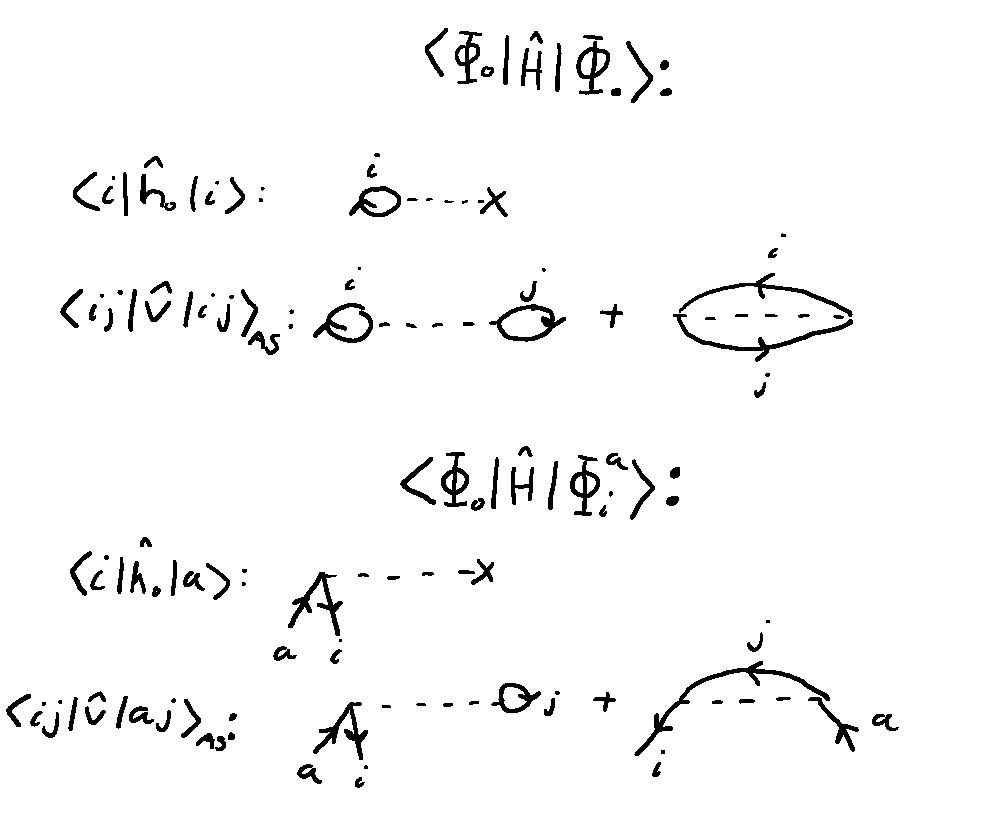
\includegraphics[width=\linewidth]{gs_1p1h_croped.pdf}
        \caption{Diagrammatic representation of matrix elements for $\inner{\Phi_0}{\hat{H}}{\Phi_0}$ and $\inner{\Phi_0}{\hat{H}}{\Phi_{i}^a}$}\label{fig:gs_1p1h}
    \end{figure}

    \begin{figure}[H]
        \centering
        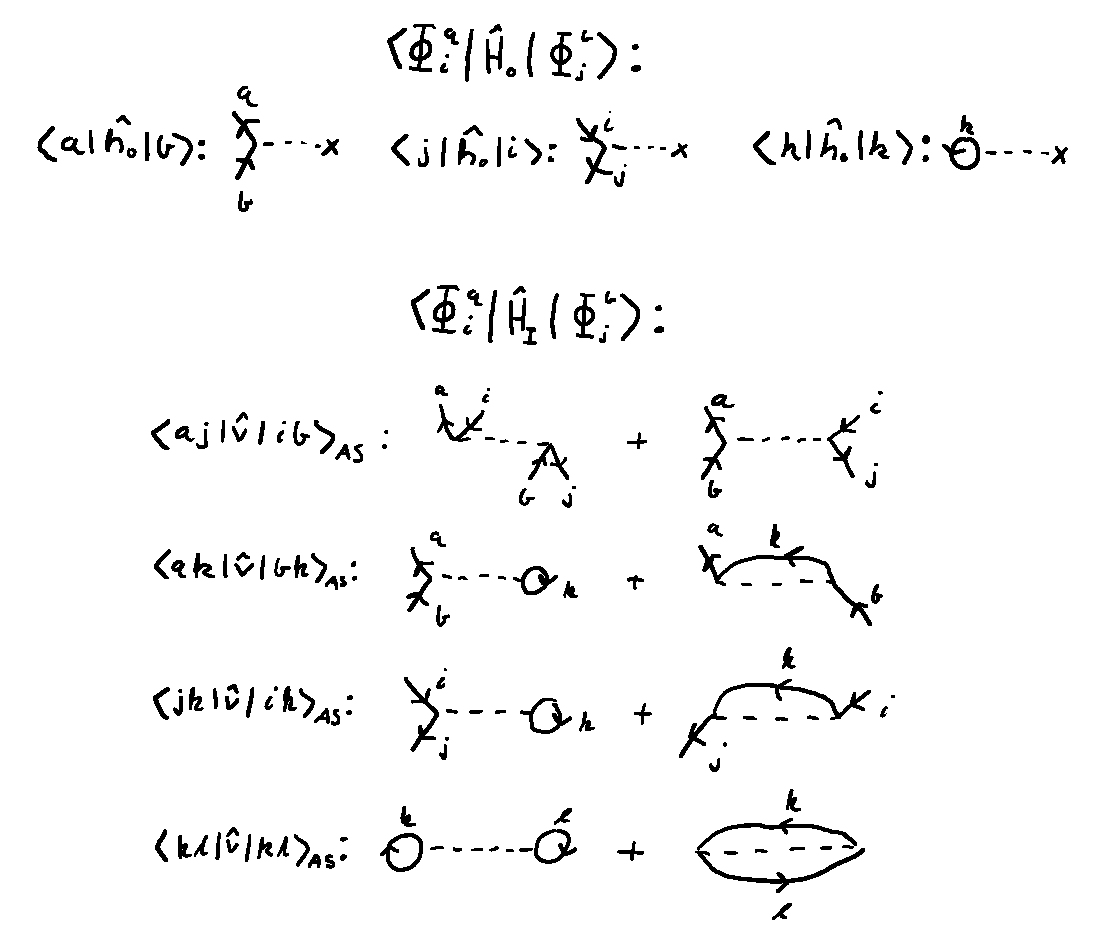
\includegraphics[width=\linewidth]{2p2h_croped.pdf}
        \caption{Diagrammatic representation of matrix elements for $\inner{\Phi_i^a}{\hat{H}}{\Phi_j^b}$, decomposed in terms for $\hat{H}_0$ and $\hat{H}_I$.}\label{fig:1p1h}
    \end{figure}
\end{appendix}
\cite{DFTgap}
\printbibliography

\end{document}

